\section{Ejercicio 2}

\subsection{Introducción}
\label{introej2}
	El segundo problema consistió en la implementación de un algoritmo capaz de dar solución al problema que se plantea a continuación:

	 Decidir si un grupo de n personas pueden formar o no una ronda que cumpla con las siguientes restricciones:
	\begin{itemize}
	      \item La ronda debe contener a todas las personas.
	      \item Algunas personas son amigas y otras no. 
	      \item Cada alumna debe tomar de la mano a dos de sus amigas.
	 
	\end{itemize}

	
\subsection{Explicación}
	Dado que para este problema no se conocen algoritmos buenos\footnote{Un algoritmo se considera bueno si puede ser resuelto en tiempo polinomial.},
	se pensó en utilizar la solución por fuerza bruta, es decir, intentar todas las combinaciones hasta lograr determinar si hay o no solución, pero, agregando 
	algunas mejoras.

	Mejoras como evaluar, en el momento de cargar la ronda, si alguna persona no tiene las suficientes amigos, es decir 2, o si todos son amigos de todos.	

	Luego, se pensó en la estrategia de ``Vuelta atrás'', (Backtracking).
\\ \\ \\
\textit{
\underline{\textbf{Backtracking:}}\\
En su forma básica, la idea de backtracking se asemeja a un recorrido en profundidad dentro de un grafo dirigido. El grafo en cuestión suele ser un árbol, o por lo menos no contiene ciclos. Sea cual sea su estructura, existe sólo implícitamente. El objetivo del recorrido es encontrar soluciones para algún problema. Esto se consigue construyendo soluciones parciales a medida que progresa el recorrido; estas soluciones parciales limitan las regiones en las que se puede encontrar una solución completa. El recorrido tiene éxito si, procediendo de esta forma, se puede definir por completo una solución. En este caso el algoritmo puede bien detenerse (si lo único que se necesita es una solución del problema) o bien seguir buscando soluciones alternativas (si deseamos examinarlas todas). Por otra parte, el recorrido no tiene éxito si en alguna etapa la solución parcial construida hasta el momento no se puede completar. En tal caso, el recorrido vuelve atrás exactamente igual que en un recorrido en profundidad, eliminando sobre la marcha los elementos que se hubieran añadido en cada fase. Cuando vuelve a un nodo que tiene uno o más vecinos sin explorar, prosigue el recorrido de una solución.
}\footnote{http:\/\/es.wikipedia.org\/}
\\ \\

En este caso particular, la idea es, seleccionar una persona (P), ingresarla en la ronda, e ir armando un arbol implicito de posibilidades en donde
el nodo padre es P y cada rama se forma con las distintas selecciones de amigas de P y sus sub-arboles, con las combinaciones posibles de amigas del nodo padre en el que esté.
Para ello se utiliza la recursión, en donde se intenta bajar lo más posible en el arbol hasta llegar a formar un camino desde el primer nodo hasta alguna hoja en donde se encuentren
todas las chicas con nodos padre e hijo amigas.

También, se implementaron otras mejoras que intentan podar el arbol dadas ciertas condiciones que permitan acortar las posibilidades:
\begin{itemize}
 \item Las amigas de un nodo se pueden procesar en cualquier orden, pero decidimos intentar ser lo más restrictivo posible con las primeras (las que tienen menos amigas primero). Este proceso poda el árbol de búsqueda antes de que se tome la decisión y se llame a la subrutina recursiva.
 \item Cuando se elige qué valor se va a asignar, se hace un examen comprobando que aún queden amigas de la que inició la ronda disponibles. En caso que no, se pueden evitar muchas llamadas sin sentido.
\end{itemize}

A continuación se ve un pseudocodigo que muestra el comportamiento de la estrategia y las mejoras elegidas.

\vspace{3cm}
\underline{Algunos detalles:}

\begin{itemize}
 \item \textbf{gente} es una lista con elementos de tipo chica, ordenadas de acuerdo a la cantidad de amigas que tiene cada elemento.
 \item el tipo \textbf{chica} consta de un nombre (int) y sus amigas (conjunto de nombres).
 \item \textbf{enRonda} es un conjunto de nombres donde se va almacenando quienes pertenecen a la ronda.
 \item \textbf{amigasPrimera} es un conjunto de nombres donde se almacenan los nombres de las amigas de la chica que comienza la ronda.
 \item \textbf{tam(c)} devuelve el tamaño del conjunto c.
 \item \textbf{insertar(c,e)} inserta a e en el conjunto c.
 \item \textbf{borrar(c,e)} borra a e del conjunto c.
 \item \textbf{cuenta(c,e)} cuenta la cantidad de apariciones del elemento e en c.
 \item \textbf{primerElemento(l)} devuelve el primer elemento de una lista.
\end{itemize}

\newpage

\incmargin{1em}
\linesnumbered
\restylealgo{boxed}

\textbf{resolver()}\\
\SetKw{Orden}{Complejidad:}
	\begin{algorithm}[H]
	\Orden{T(n)}
		\BlankLine
		\textbf{var} n : int $\leftarrow$ tam(gente) \\
		\textbf{var} sonPocas : bool $\leftarrow$ false \\
		\textbf{var} sonSuficientes : bool $\leftarrow$ false \\
		
	  \ForEach{k en gente}{
		  sonPocas $\leftarrow$ sonPocas or tam(amigas(k)) $<$ 2;\\
		  sonSuficientes $=$ sonSuficientes $\&\&$ tam(amigas(k)) $==$ n-1);
	   }
    \If{(sonSuficientes)}{retornar true}
    \If{(sonPocas)}{retornar false}

	\textbf{var} solitaria : chica $\leftarrow$ primerElemento(gente);

	insertar(nombre(solitaria),enRonda);

	retornar  probarDistintasRondas(solitaria,solitaria);
	\BlankLine




	  \end{algorithm}
	  


%segundo algoritmo:
\incmargin{1em}
\linesnumbered
\restylealgo{boxed}

\textbf{probarDistintasRondas(prim : chica, ult : chica)}\\
\SetKw{Orden}{Complejidad:}
	\begin{algorithm}[H]
	\Orden{T(n)}
		\BlankLine
	\eIf{(cuenta(amigas(ult),nombre(prim)) $\neq$ 0 $\&\&$ tam(gente) $=$ tam(enRonda) )}{retornar true;}{
		\textbf{var} res : bool\\
		\textbf{var} eraAmiga : bool $\leftarrow$ false \\
\BlankLine		
\ForEach{chi en gente}{
		\textbf{var} estaEnRonda : int $\leftarrow$ cuenta(enRonda,nombre(chi)) \\
		\textbf{var} esAmigaDeLaUltima : int $\leftarrow$ cuenta(amigas(ult),nombre(chi)) \\
		\textbf{var} restantesAmigasPrimera : int $\leftarrow$ tam(amigasPrimera) \\
		\textbf{var} esAmigaDeLaPrimera : int $\leftarrow$ cuenta(amigas(prim),nombre(chi)) \\
		  \BlankLine
	\If {( (estaEnRonda $=$ 0) $\&\&$ (esAmigaDeLaUltima $\neq$ 0) $\&\&$ (restantesAmigasPrimera $\neq$ 0) )}{
\BlankLine	
			\eIf{(esAmigaDeLaPrimera $\neq$ 0)}{
					eraAmiga $\leftarrow$ true;\\
					eliminar(amigasPrimera,nombre(chi));
				}{
					eraAmiga $\leftarrow$ false;
				}
				insertar(enRonda,nombre(chi));\\
				res $\leftarrow$ probarDistintasRondas(prim,chi);
\BlankLine	
			\eIf{(res)}
				{
					retornar true;
				}
				{
					borrar(enRonda,nombre(chi));\\
\BlankLine	
				\If{(eraAmiga)}{insertar(amigasPrimera,nombre(chi))}
						}
				}	
		}
		retornar false;
	}	


  \end{algorithm}



\subsection{Análisis de la complejidad del algoritmo}
\label{complejidadej2}

\paragraph{}
La complejidad en el peor caso de este algoritmo surge inmediatamente al hacer pruebas. Dependiendo de las entradas elegidas, el programa podría tener que 
recorrer casi todas las ramas del árbol hasta poder decir que no hay solución. En este caso, podríamos entonces solo acotar el peor caso por la función $f(n) = c.(n-1)! + b$ 
(donde b y c son constantes) ya que la cantidad de formas de armar una ronda con n personas es (n!/n) = (n-1)!\footnote{Se lo puede imaginar como una fila de n personas. Para la primer posición hay n personas disponibles, para la segunda n-1, y así sucesivamente. Por lo tanto hay n*(n-1)*...*1 = n! formas de acomodar las personas en una fila. Ahora, si se unen las puntas, podría rotar la fila n veces y seguiría siendo la misma ronda, por lo tanto dividiendo por n obtengo la respuesta: \textbf{(n-1)!}.} 

\paragraph{}
Por lo tanto, el algoritmo implementado NO es bueno. Sin embargo, cuando para un conjunto de datos de entrada se puede formar una ronda, el algoritmo no recorre todo el árbol en busca de la solución, sino que al encontrar una termina. Esta propiedad del backtracking y el resto de las mejoras, hace que para ciertos datos de entradas en donde se pueden formar rondas, el algoritmo se comporte como lo haría una solución polinomial.

\paragraph{}
En lo que respecta a la complejidad del mejor caso, se puede ver de forma simple que el mismo se da si en el primer intento de formar una ronda se lograra llegar a una respuesta válida. Esto significa que el algoritmo demoró $n$ pasos para unir a las amigas y uno más para verificar que era una ronda válida. Por lo tanto, la complejidad en el mejor caso es \omegade{n} \footnote{esta cota menor se podría dar optimizando el algoritmo para que se comporte de la manera descripta pero sin algunas mejoras como comprobar para adelante en cada paso por ejemplo.}


\subsection{Detalles de Implementación}
\paragraph{}
Para compilar este programa, sólo hace falta ejecutar el comando make. El modo de uso del mismo es simple: En la carpeta que contiene al ejecutable debe existir un archivo con los datos de entrada llamado ``entrada''. El programa pasará a ejecutarse al escribir .\/main en la consola y una vez que termine, devolverá en un archivo llamado ``salida'' el resultado buscado.

Si se desean generar casos de pruebas, se puede utilizar el generador que se encuentra dentro de la carpeta del ejercicio 2, en la subcarpeta otros.

Este generador se puede compilar utilizando el comando ``g++ main.cpp'' en la consola de linux, y luego ejecutandolo con el comando .\/a.out

Una vez abierto, el programa solicita un porcentaje $(0 \leq porc \leq 100)$ y un numero maximo de chicas (max), el funcionamiento es el siguiente:

Se generan rondas de tamaño 2, 3, 4, ..., max inclusive, en donde en cada una, el programa intenta formar aproximadamente $(porc/100)*numeroTotalDeConecciones$ de amistades. Es decir, para $n$ chicas, hay $n$.$(n-1)/2$ rondas amistades posibles, por lo tanto, el programa intentara formar $(porc/100)*(n*(n-1)/2)$ amistades en la ronda.

Este programa genera un archivo con el nombre ``entradap'', que puede ser utilizado como entrada para el programa principal (cambiandole el nombre por ``entrada'').


Si se desea medir el tiempo que demora el algoritmo para una entrada, se puede utilizar el programa almacenado en la carpeta Ej2\/otros\/Tiempos.

Los pasos a seguir son equivalentes a los del programa original, necesita una entrada ``entrada'' y ser compilado con la instruccion make. 
luego con .\/main 

\subsection{Resultados}
\label{resultadosej2}


	\begin{table}[ht] %ubicacion de la tabla
		\centering %centra la tabla
			\begin{tabular}{c}
				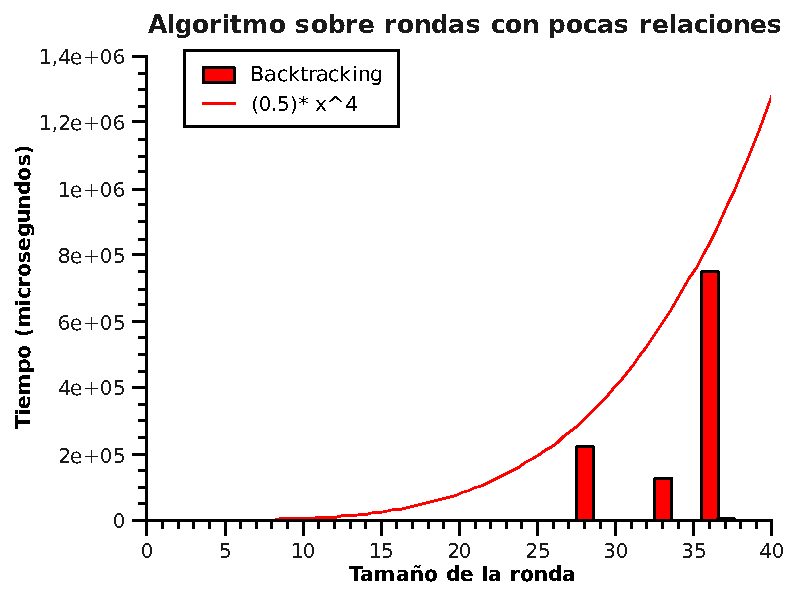
\includegraphics[scale=0.7]{../Ej_2/Otros/Graficos/Graph10-1.pdf} \\
				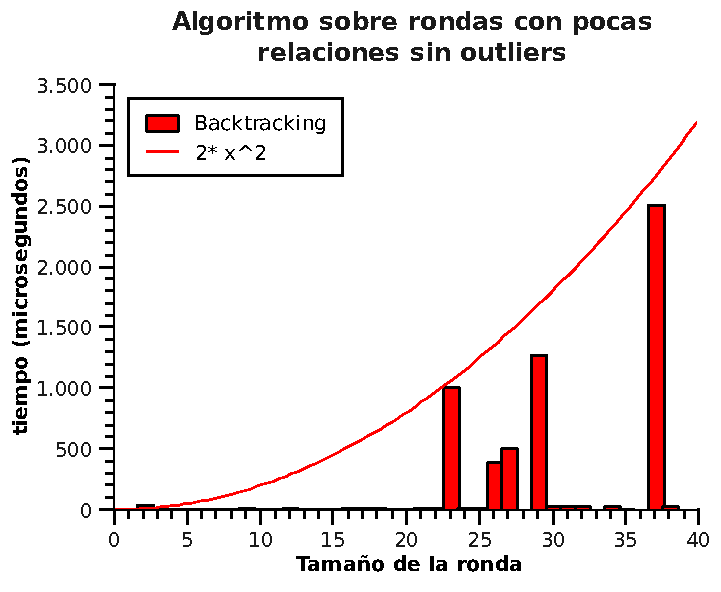
\includegraphics[scale=0.7]{../Ej_2/Otros/Graficos/Graph10-2.pdf}
				\end{tabular}
				\caption{Rondas con pocas relaciones: Estos graficos muestran la desigualdad entre tiempos de resolución para rondas es donde es complicado encontrar la solución. Se ve que quitando unos pocos outliers, los tiempos se encuentran en otros ordenes. Para ver este suceso, basta con obvservar las escalas de tiempo (en un gráfico se mueve entre 0 y 3500 microsegundos, y en la que posee outliers entre 0 y 1400000 microsegundos.) o también se puede observar las funciones que se utilizaron para dar cuenta de las dimensiones (en una comparada con $0.5*x^4$ y en la otra con $2x^2$).} %titulo de la tabla
				\label{tiempoEj2a} %con esto puedo referenciar a la tabla \ref{Tiempo metodos}
	\end{table}

	\begin{table}[ht] %ubicacion de la tabla
		\centering %centra la tabla
			\begin{tabular}{c}
				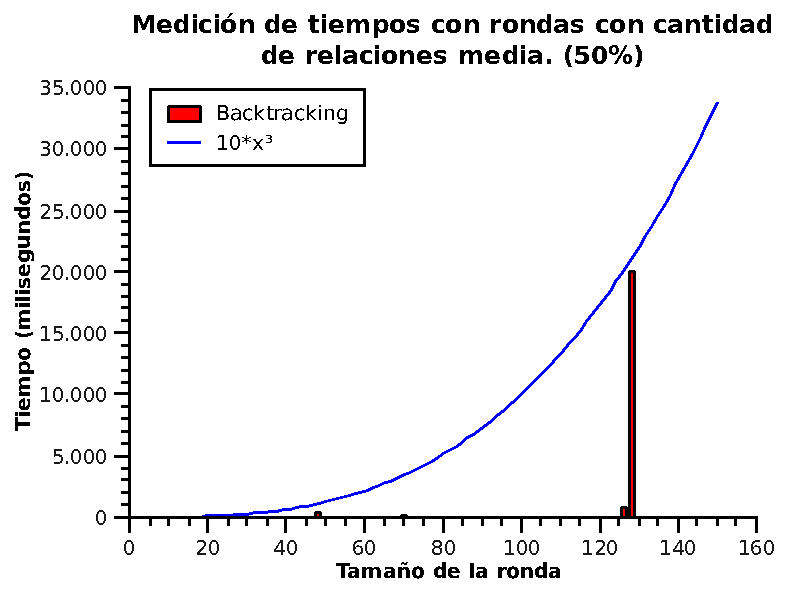
\includegraphics[scale=0.7]{../Ej_2/Otros/Graficos/Graph50-1.pdf} \\
				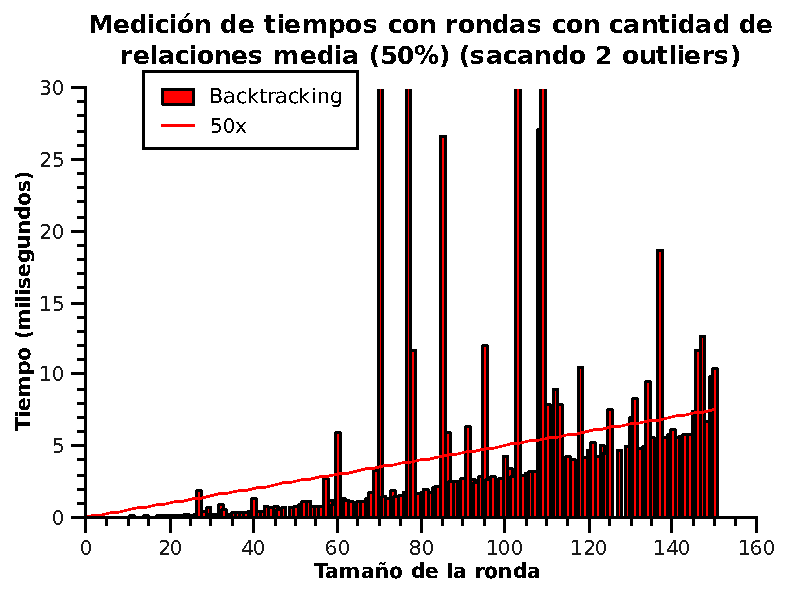
\includegraphics[scale=0.7]{../Ej_2/Otros/Graficos/Graph50-2.pdf}
			\end{tabular}
			\caption{Rondas con una cantidad media de relaciones: En estos se puede observar como 2 outliers destruyen el caso promedio que se venia dando en el tiempo de resolución del algoritmo, pasando de graficos que se comparan con $10*x^3$ contra otro que compara con $50*x$, es decir, para rondas donde hay buenas probabilidades de que se pueda formar, el algoritmo parecería comportarse linealmente, pero claramente es una ilusión.} %titulo de la tabla
			\label{tiempoEj2b} %con esto puedo referenciar a la tabla \ref{Tiempo metodos}
	\end{table}

\begin{table}[ht] %ubicacion de la tabla
\centering %centra la tabla
\begin{tabular}{c}
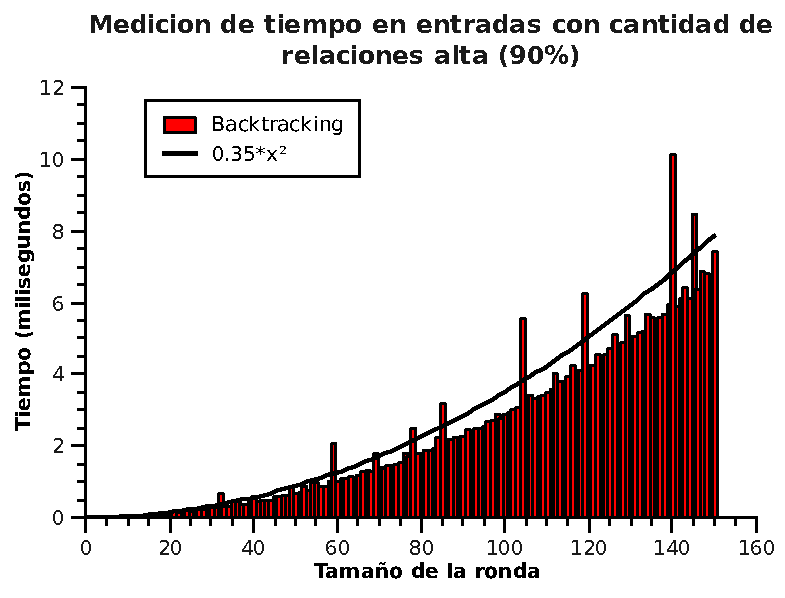
\includegraphics[scale=0.7]{../Ej_2/Otros/Graficos/Graph90.pdf} \\
\end{tabular}

\caption{Rondas con una cantidad alta de relaciones: Cuando es muy poco probable que NO se pueda armar una ronda, el algoritmo y sus mejoras claramente funcionan bien (polimomial), como es el caso de este gráfico. Esto se debe a las propiedades del backtracking y a las mejoras implementadas.} %titulo de la tabla
\label{tiempoEj2c} %con esto puedo referenciar a la tabla \ref{Tiempo metodos}
\end{table}




\subsection{Debate}
\paragraph{}
De los resultados pertenecientes a la sección [\ref{complejidadej2}] podemos observar cómo se comporta la implementación frente a algunas entradas particulares. Las mismas fueron creadas al azar pero de forma tal que se cumplan los invariantes citados en [\ref{introej2}] y con el agregado de fijar la cantidad de enlaces (amistades) en cada ronda (esta función del generador de casos de prueba es explicado en la sección \textbf{detalles de implementación}.


\paragraph{}
En un primer análisis, podemos ver que en general para todos los casos analizados la función proveniente de graficar cantidad de chicas contra tiempo demorado en ejecutar el algoritmo se asemeja bastante a una función polinomial cuando la cantidad de relaciones es alta. Si bien sabemos que esto no refleja la verdadera complejidad del algoritmo, en primer instancia podría significar un buen funcionamiento de las mejoras realizadas sobre el algoritmo.

\paragraph{}
La función antes mencionada, pareciera ser bastante monótona. Igualmente, se observa con claridad la aparición de casos en los cuales se demoró mucho más tiempo que el tiempo promedio. Esto podría dejar entrever que para ciertos valores de la entrada o no se encontró resultado alguno, por lo cuál se tuvieron que analizar los (n-1)! casos posibles, o bien se encontró una solución al problema, pero esta se demoró en ser encontrada ya que se trataba de un ejemplo en el cual las mejoras realizadas no surtieron efecto o, peor aún, tuvieron un efecto contrario al deseado.


\subsection{Conclusiones}

\paragraph{}
Como resultado del análisis de los datos arrojados en [\ref{resultadosej2}] y de las hipótesis realizadas anteriormente, podemos concluir:.

Primero, para muchos de los casos analizados durante el transcurso de este trabajo práctico, el algoritmo llegó a una respuesta en un tiempo promedio mucho menor al que en teoría debería demorar. Por lo tanto, podemos intuir que las mejoras realizadas dentro del algoritmo fueron, en general, muy productivas. Sin embargo, no nos aseguran que el algoritmo mejore su complejidad asintóticamente.

\paragraph{}
En segundo lugar, y continuando lo antes dicho, se observaron casos en los cuales el algoritmo demoró más que el tiempo promedio. Esto puede deberse a que, para ciertos casos de entrada, las mejoras del algoritmo no inciden en la resolución del problema, haciendo que se demore demasiado en conseguir una solución válida. Si se suma el hecho de analizar dichos casos para entradas de gran tamaño, podemos llegar a estar ante un problema, ya que el tiempo de resolución del problema para nuestro algoritmo puede ser, en términos humanos, eterno.

\paragraph{}
Finalmente, podemos concluir entonces que el algoritmo, más allá de las mejoras implementadas sobre el mismo, no alcanza a obtener una complejidad de peor caso menor que \Ode{n!}, pero las mismas sirven para que el algoritmo encuentre más fácilmente el camino hacia una buena solución\footnote{Siempre y cuando exista al menos una solución al problema y además, esta solución se condiga con las mejoras elegidas en la implementación.}.

